% !TEX root =  ../supplementary.tex
\section{Web-Application for Practical Use of Personalized Schedule of Biopsies}

We implemented our methodology in a web-application to assist patients and doctors in better decision making. It works on desktop as well as mobile devices. The cohorts that are currently supported in this web-application are PRIAS and the largest six cohorts from the GAP3 database \citep{gap3_2018}. These are the University of Toronto AS (Toronto), Johns Hopkins AS (Hopkins), Memorial Sloan Kettering Cancer Center AS (MSKCC), King's College London AS (KCL), Michigan Urological Surgery Improvement Collaborative AS (MUSIC), and University of California San Francisco Active Surveillance (UCSF). The web application is hosted at \url{https://emcbiostatistics.shinyapps.io/prias_biopsy_recommender/}. 

\begin{figure}[!htb]
\centerline{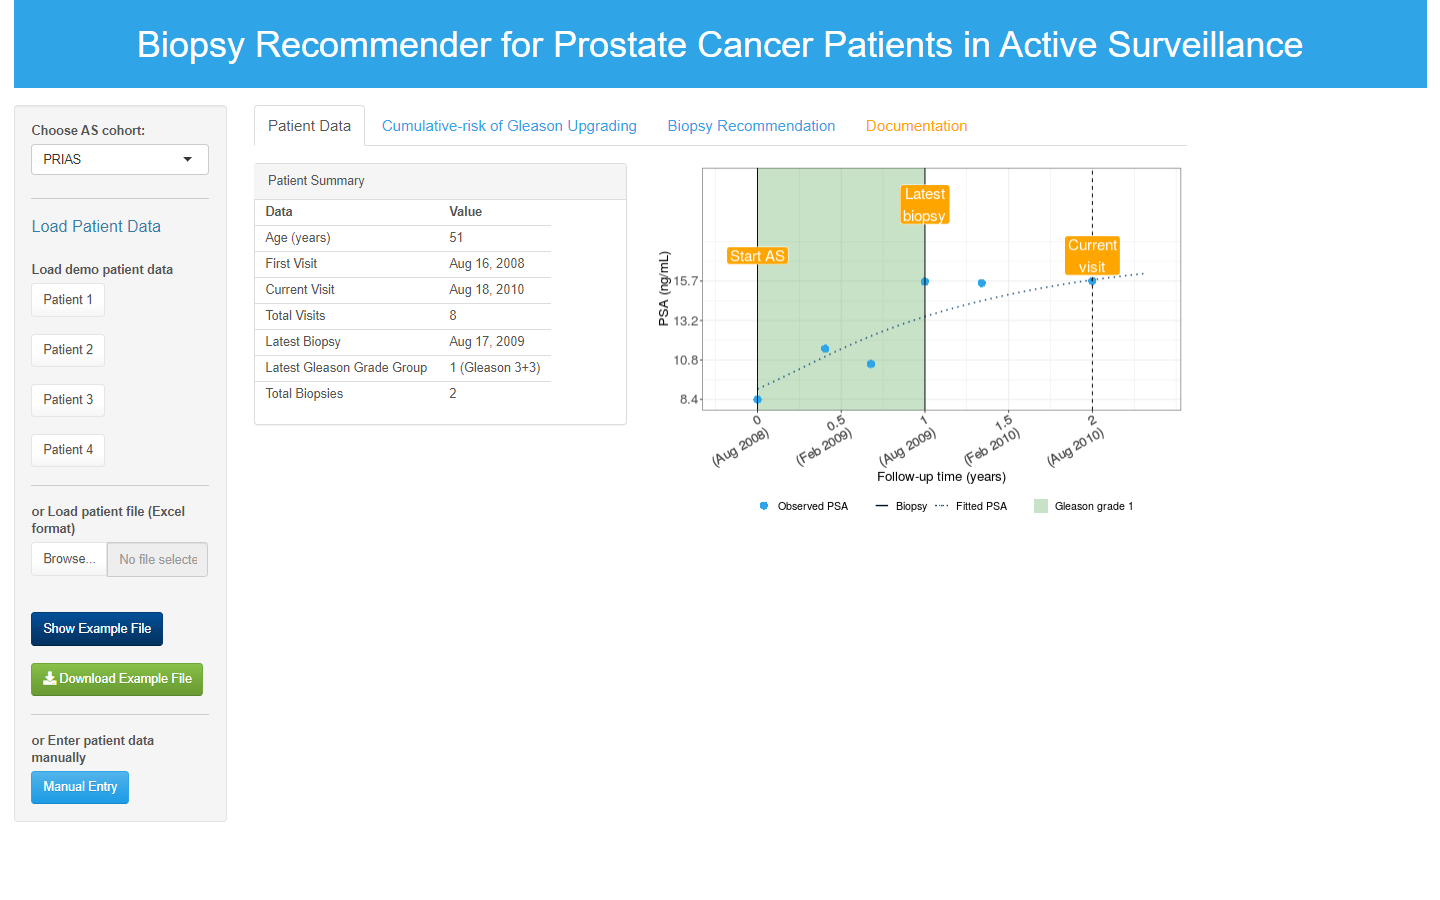
\includegraphics[width=\columnwidth]{images/app/landing_page.png}}
\caption{Landing page of the web-application. Panel on the left allows users to load patient data and panel on the right provides information. Patient data can be entered manually, or via Excel files. In addition, demo patient data is already uploaded to assist users in understanding the web-application.}
\label{fig:landing_page}
\end{figure}